\section{Experiments}

In this section, we conduct experiments to evaluate the effectiveness of our proposed visual features in section \ref{sec_vis_feature}.

\subsection{Datasets Description}

Wikimedia provides public dumps for content on Wikipedia. We refer to both Wikipedia dumps and clickstream as our datasets. Datasets on Wikipedia are representative due to the significant data quantity and the variety of users, editors and contents. Wikipedia datasets are released monthly. In this work, we focus on the English version released in March 2021.

\subsubsection {Wikipedia Pages}

The page contents on Wikipedia are available in the format of public dumps. We process all the English articles from Wikipedia XML dump \footnote{https://dumps.wikimedia.org/backup-index.html}. We focus on all articles contained in the main namespace of the English Wikipedia. There are more than 5 million articles in the March 2021 release, reaching 60GB of text in total. To obtain rendered visual features in \cite{dimitrov2017makes}, we retrieved the Html pages through a public Wikipedia API \footnote{https://www.mediawiki.org/wiki/API:Main\_page}.

\subsubsection{Wikipedia Clickstream}

We refer to the Wikipedia clickstream dataset \footnote{https://meta.wikimedia.org/wiki/Research:Wikipedia\_clickstream} for the click log of the hyperlinks. The clickstream dataset contains transition data extracted from Wikipedia request logs. To be specific, there are many (referrer, resource) pairs in this dataset, and each one shows raw counts on the volume of traffic between the article pairs. A referrer is an Http header field that identifies the address of the webpage that is linked to the resource being requested. To reduce noise, any (referrer, resource) pair with ten or fewer observations was removed from the dataset.

To obtain the internal navigation data in Wikipedia, we exclude all the outside transitions from the dataset. The clickstream dataset can be modeled as a graph, where nodes are the articles and edges represent the transitions between articles. There are a total of 32M (referrer, resource) pairs in the March 2021 release \footnote{https://dumps.wikimedia.org/other/clickstream/2021-03}.

\subsection{Experimental Setup and Metrics}

Despite the huge size of the dataset, we can only use a small fraction for the experiments. The reason is that only about 4\% of hyperlinks on Wikipedia get clicked more than 10 times within a month, indicating the scarcity of the click data. We pick the top 50,000 most frequently clicked articles as our dataset to avoid low-quality data. To obtain experimental results under different domains, we partition the dataset by categories defined by Wikipedia. We construct a tree-like structure to represent the category relationships. Then, we run Breadth-first search algorithm to classify each article into one of the 41 categories according to its shortest distance from these main categories. In our experiments, we only pick the category with more than 1000 articles for data quantity. Each of the ten datasets is randomly partitioned for different purposes: 60\% of articles are used for training, 20\% for validation, and the rest 20\% is for testing.

For Learning to Rank, we adopt a Python implementation \footnote{https://github.com/jma127/pyltr} of LambdaMart \cite{wu2010adapting} in our experiments. Two metrics are used for evaluating different features: Normalized Discounted Cumulative Gain (NDCG) and Expected Reciprocal Rank (ERR).

\subsection{Baseline Features}

We introduce two baselines \cite{thruesen2016link, dimitrov2017makes} for comparison. To be specific, the first baseline \cite{dimitrov2017makes} used textual feature \#1,2 in Section \ref{textual_features}, graph-based features \#1,2,3 in Section \ref{graph-based_features} and all the render features in Section \ref{render_features}. Besides, the second baseline \cite{thruesen2016link} utilized textual features \#1,3,4,5,6 and graph-based features \#3,4,5,6,7. As for our method, we adopt all the visual features, textual features and graph-based features.

\subsubsection{Textual Features} \label{textual_features}

The following textual features are used for ranking. We use $source$ and $dest$ to respectively denote the article the user is reading, and the article the hyperlinking is directing to.

\begin{itemize}

    \item[1.] \emph{Text Similarity}: Cosine similarity of TF-IDF vectors between texts in $source$ and $dest$.

    \item[2.] \emph{Topic similarity} (\cite{dimitrov2017makes}): Cosine similarity of embedding vectors between Wikipedia categories assigned to $source$ and $dest$.

    \item[3.] \emph{Order}: The $x$th hyperlink in the text.

    \item[4.] \emph{Number of links}: The number of times the hyperlink appears in the article. 

    \item[5.] \emph{Position} and \emph{Log of Position}: \emph{Position} and \emph{Log of Position} represents the absolute and relative positions of hyperlinks in the article text.

    \item[6.] \emph{Topic similarity} (\cite{thruesen2016link}) : The Jaccard coefficient of titles words in
    source and dest, which represents the similarity between two titles

\end{itemize}

\subsubsection{Graph-based Features} \label{graph-based_features}

All the articles together can be modeled as a graph. We introduce the following graph-based features.

\begin{itemize}

    \item[1.] \emph{In\_Degree}, \emph{Out\_Degree} and \emph{Degree}: The in degree, out degree and degree of the article.

    \item[2.] \emph{K-Core Score}: Score computed by K-Core measure.

    \item[3.] \emph{PageRank Score}: Score computed by Pagerank algorithm \cite{brin1998anatomy}.

    \item[4.] \emph{Symmetric link}: The feature takes value from $\{0,1\}$, indicating whether or not the link is symmetric. A link $(source, dest)$ is considered symmetric if and only if the corresponding link $(dest, source)$ also exists. 

    \item[5.] \emph{Hub Score} and \emph{Authority Score}: Both Hub Score and Authority Score are calculated via HITS algorithm \cite{kleinberg1998authoritative}.

    \item[6.] \emph{Link Relatedness}: The similarity between link sets of $source$ and $dest$, which contains their linked articles. Two metrics are computed by Jaccard coefficient and Dice's measure.

    \item[7.] \emph{Community Detection}: Community features are obtained through three community detection algorithms: Fast greedy \cite{clauset2004finding}, Label propagation \cite{raghavan2007near}, and InfoMAP \cite{rosvall2009map}.

\end{itemize}

\subsubsection{Render Features} \label{render_features}

The last feature group is visual features from \cite{dimitrov2017makes}. To disambiguate between our proposed visual features in this paper, we name these previously proposed features as \emph{render features}.

\begin{itemize}
    \item[1.] \emph{Lead or Body}: Whether the link is positioned in the lead section.

    \item[2.] \emph{Left or Right}: Whether the link is positioned in the left 10\% of the screen.

    \item[3.] \emph{Infobox}: Whether the link is placed within the Infobox.

    \item[4.] \emph{Navbox}: Whether the link is placed within the Navbox.

    \item[5.] \emph{screen x coord}: The x coordinate of the link.
    
    \item[6.] \emph{screen y coord}: The y coordinate of the link.
    
\end{itemize}

\subsection{Results}

First, we compared our proposed visual features with previous works. The results for source link and target link are presented in Figure \ref{table_cmp1} and Figure \ref{table_cmp2}. As is shown in these two figures, there is a consistent improvement in Learning to Rank accuracy for our method. Our feature can achieve the best result among all the categories.

Then, we test each group of features alone. As we can see from Figure \ref{table_cmp3} and \ref{table_cmp4}, the group of textual features can always achieve the best result. As texts are one of the basic components of web pages, textual features are very effective in predicting the click frequencies of hyperlinks. Overall, the visual feature can achieve better results than the rest two feature groups, which validates the effectiveness of visual information. It is also worth mentioning that the render feature group gets the worst result for the target link task. It would thus be sub-optimal to incorporate such features in the Learning to Rank model. For source link ranking, the graph feature groups achieve the worst result, which indicates that graph features of source pages are less effective than target pages.


\begin{figure*}[t]
\centering
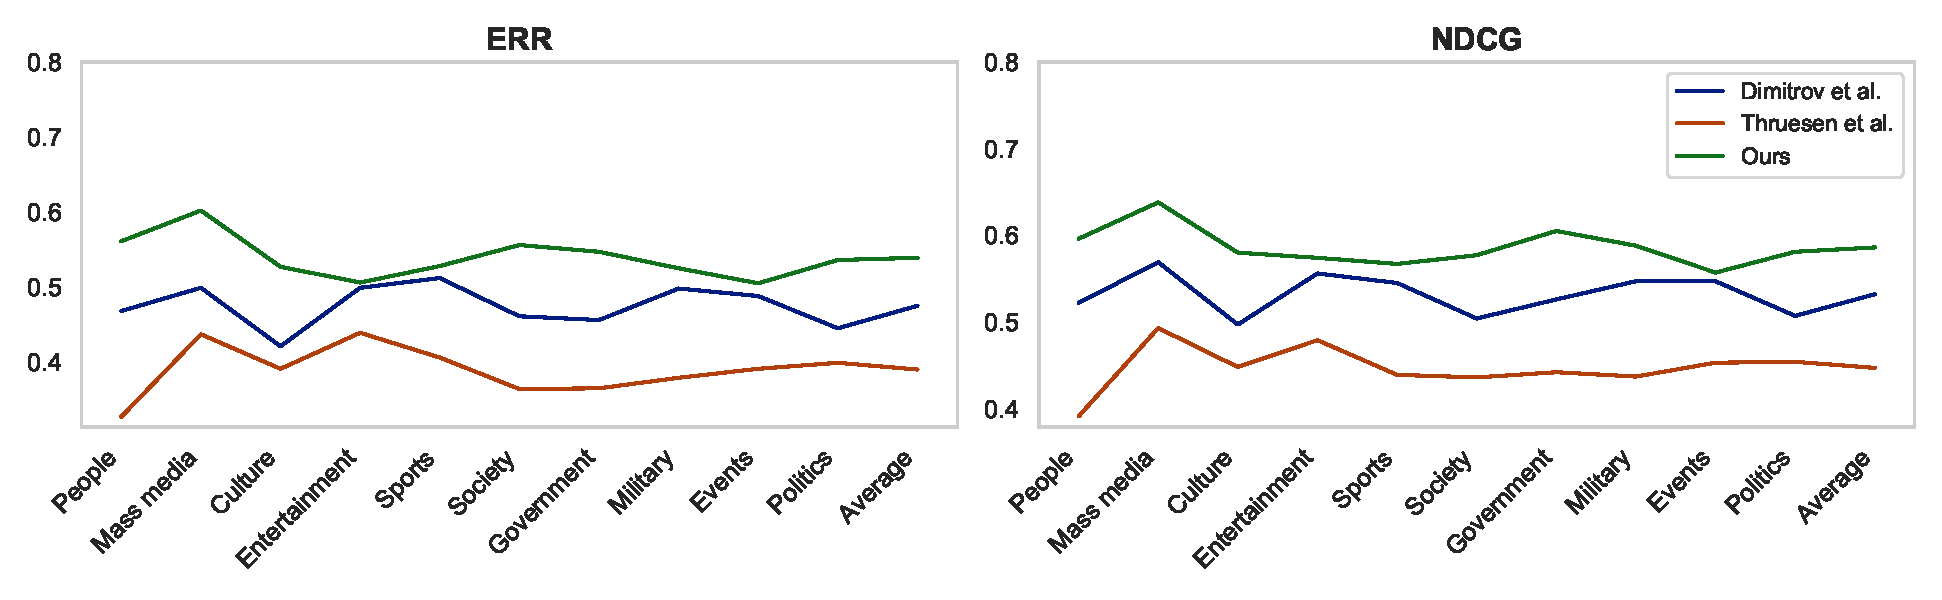
\includegraphics[width=1\textwidth,height=3.5cm]{exp_tab1_src}
\caption{Comparison with previous methods (Source link).}
\label{table_cmp1}
\end{figure*}

\begin{figure*}[t]
\centering
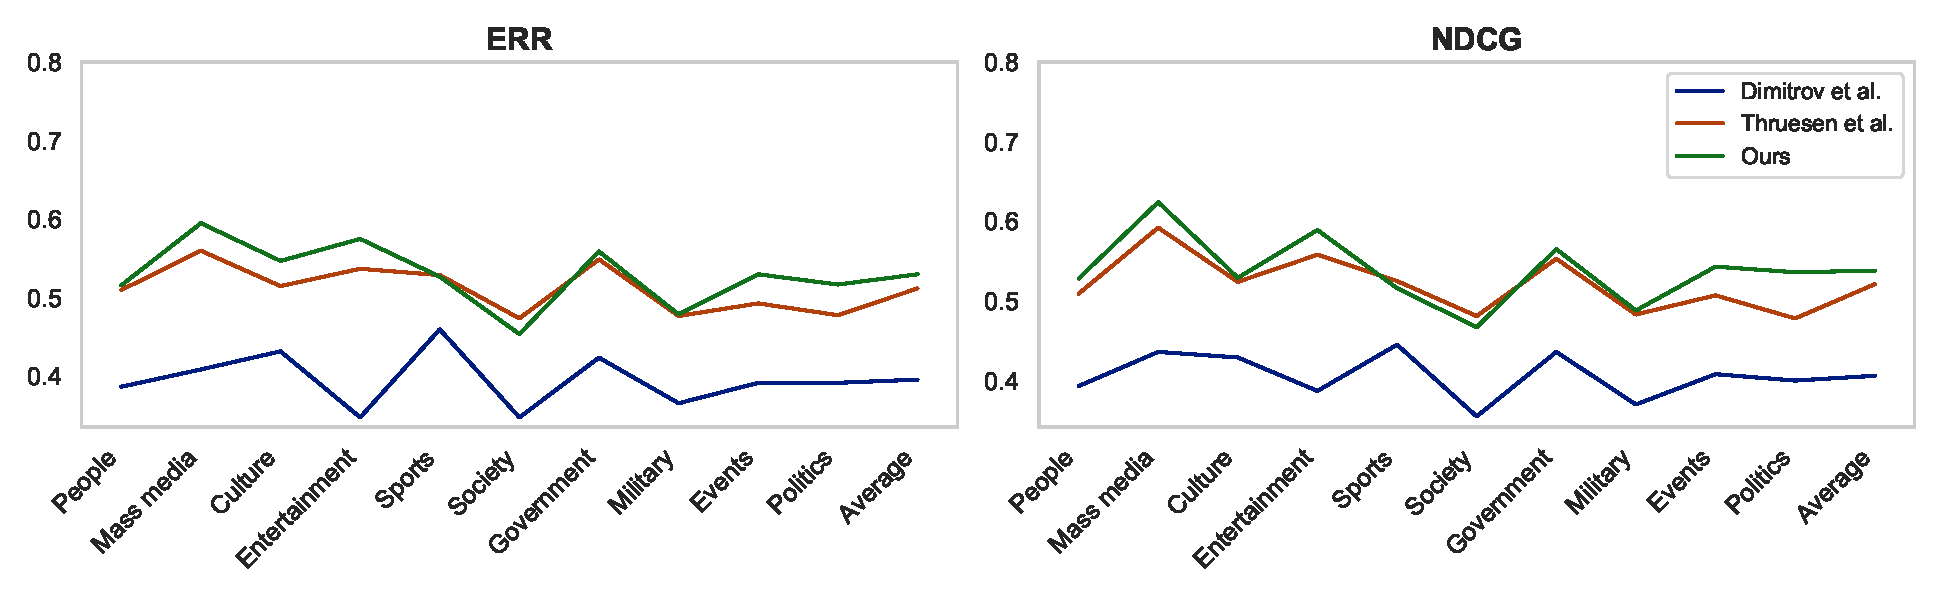
\includegraphics[width=1\textwidth,height=3.5cm]{exp_tab1_tgt}
\caption{Comparison with previous methods (Target link).}
\label{table_cmp2}
\end{figure*}

\begin{figure*}[t]
\centering
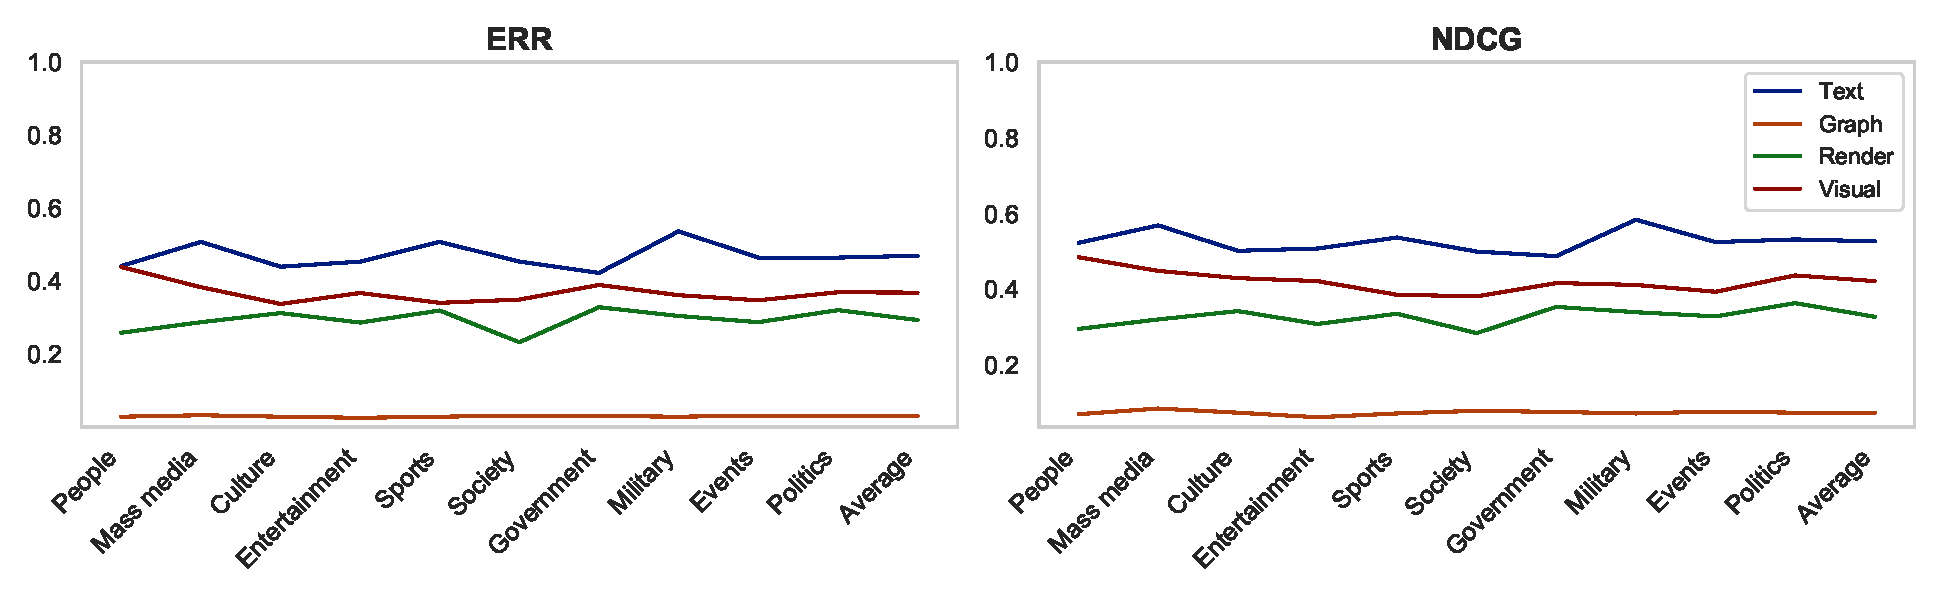
\includegraphics[width=1\textwidth,height=3.5cm]{exp_tab2_src}
\caption{Comparison between different feature groups. Render features are obtained under 1366$\times$768 resolution (Source link).}
\label{table_cmp3}
\end{figure*}

\begin{figure*}[t]
\centering
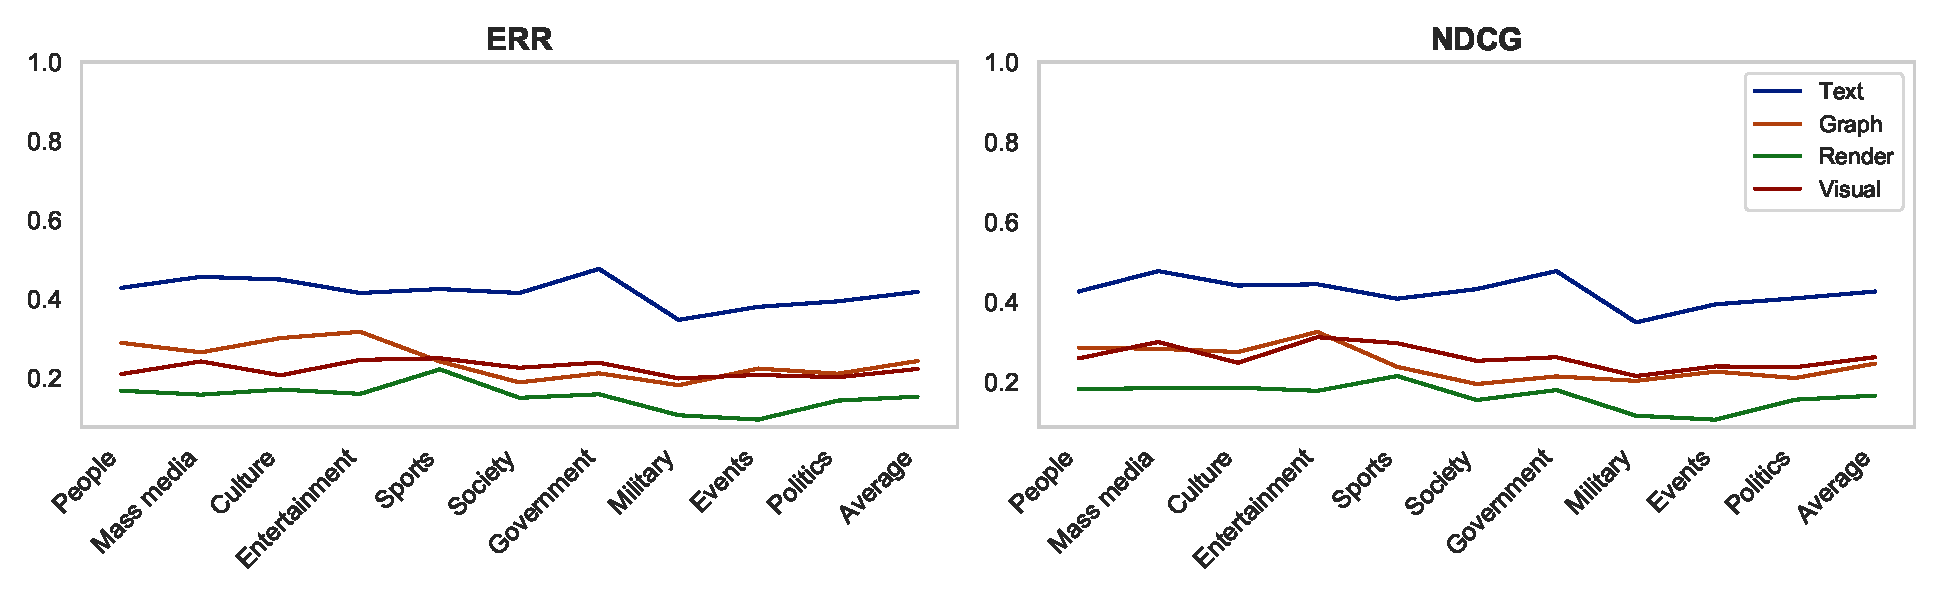
\includegraphics[width=1\textwidth,height=3.5cm]{exp_tab2_tgt}
\caption{Comparison between different feature groups. Render features are obtained under 1366$\times$768 resolution (Target link).}
\label{table_cmp4}
\end{figure*}

\begin{figure*}[t]
\centering
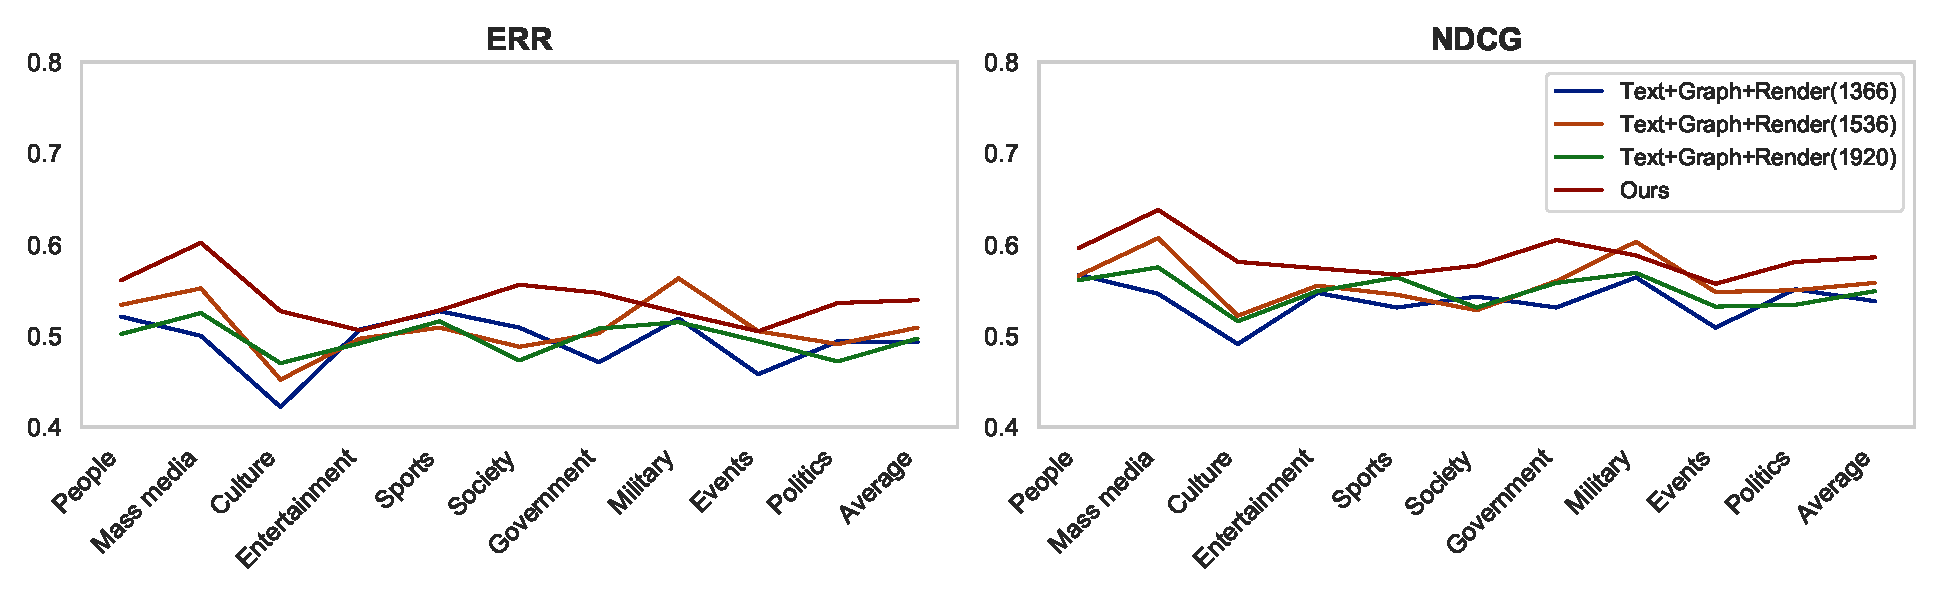
\includegraphics[width=1\textwidth,height=3.5cm]{exp_tab3_src}
\caption{Comparison between different resolutions. Render(1366), Render(1536) and Render(1920) respectively refers to the render features obtained under resolution setting 1366$\times$768, 1536$\times$864 and 1920$\times$1080 (Source link).}
\label{table_cmp5}
\end{figure*}

\begin{figure*}[t]
\centering
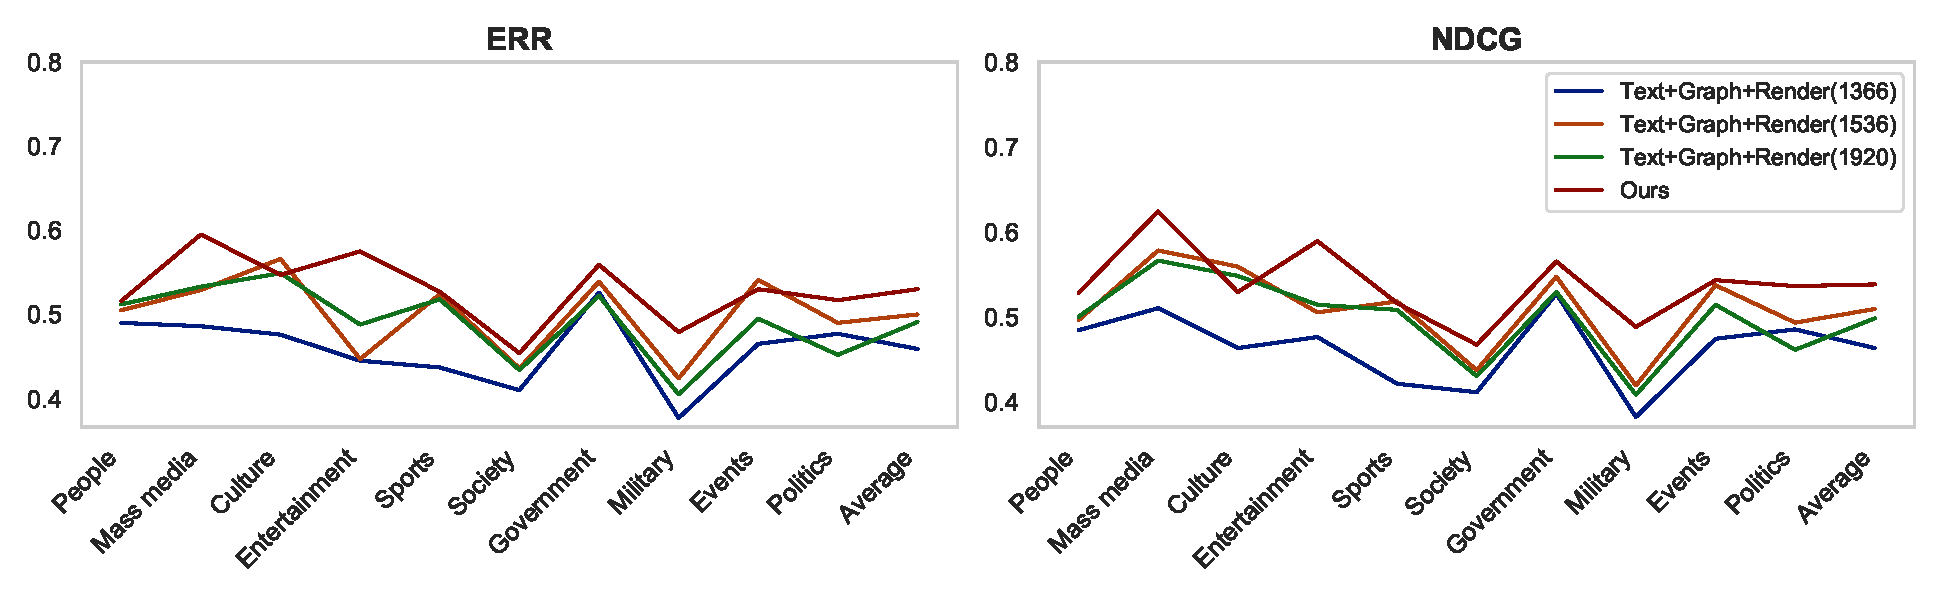
\includegraphics[width=1\textwidth,height=3.5cm]{exp_tab3_tgt}
\caption{Comparison between different resolutions (Target link). Resolution settings are the same as Table \ref{table_cmp5}.}
\label{table_cmp6}
\end{figure*}

\begin{figure*}[t]
\centering
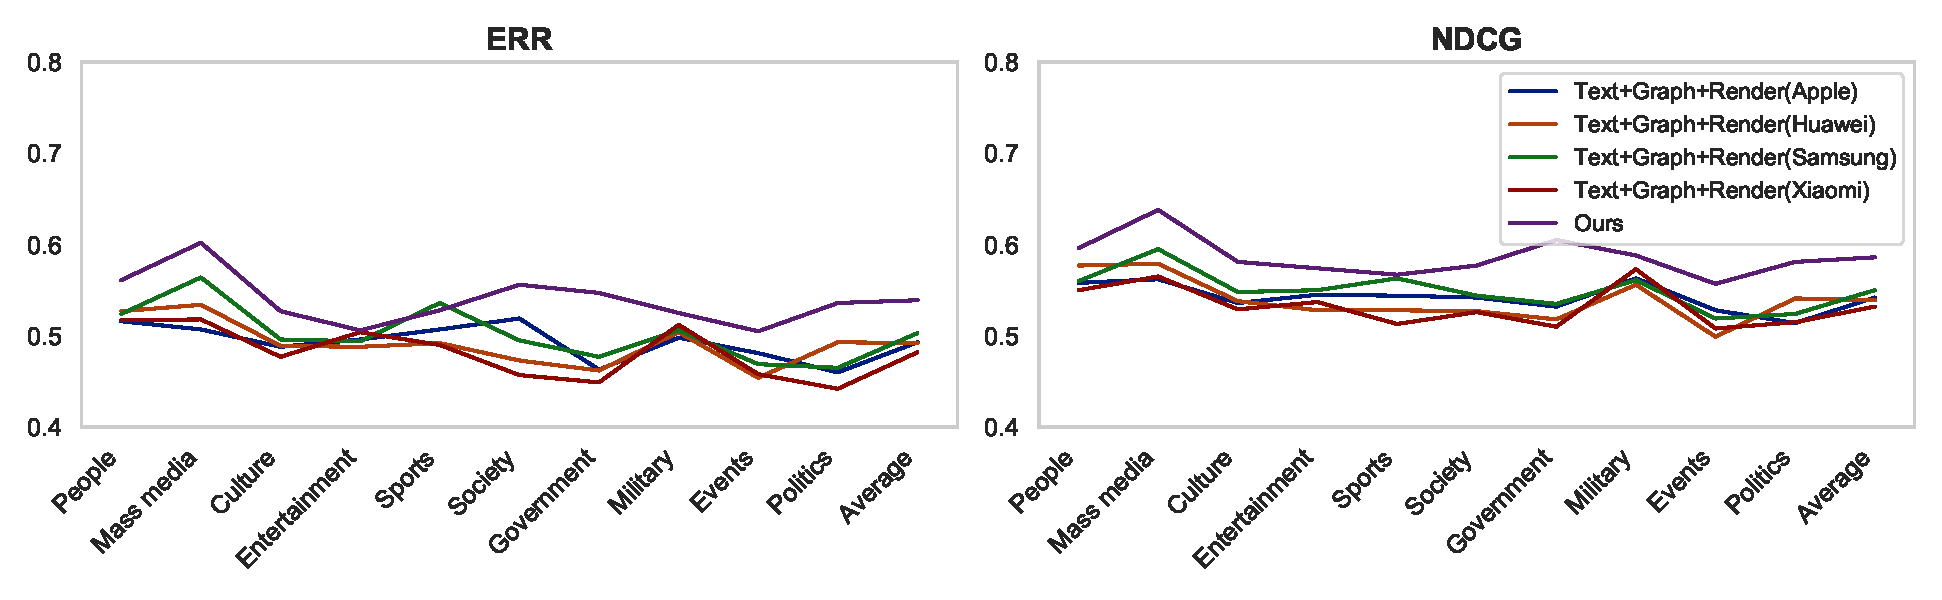
\includegraphics[width=1\textwidth,height=3.5cm]{exp_tab4_src}
\caption{Comparison with different mobile devices. Render(Apple), Render(Huawei), Render(Samsung) and Render(Xiaomi) respectively refers to the render features obtained under IPhone 12, Galaxy S10, Xiaomi Mi 10 and Huawei P40 (Source link).}
\label{table_cmp7}
\end{figure*}

\begin{figure*}[t]
\centering
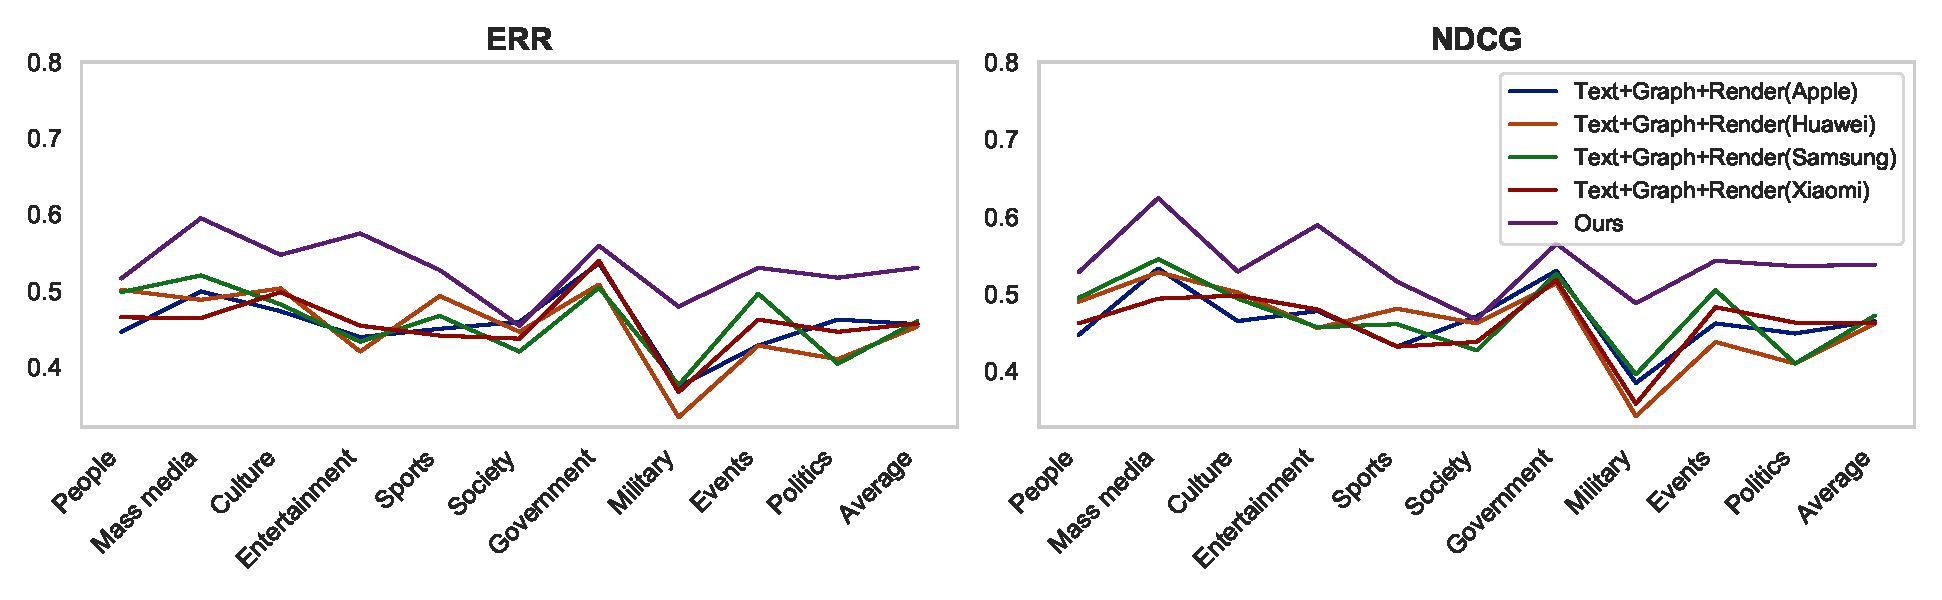
\includegraphics[width=1\textwidth,height=3.5cm]{exp_tab4_tgt}
\caption{Comparison with different mobile devices (Target link). Device settings are the same as Table \ref{table_cmp7}.}
\label{table_cmp8}
\end{figure*}

We further compare the effectiveness of our visual features and render features under different devices. We combine render features with both textual features and graph-based features for comparison. For the PC setting, we tested three resolutions ($1366x768$, $1536x864$ and $1920x1080$). According to Figure \ref{table_cmp5} and Figure \ref{table_cmp6}, our visual feature yields better results than render features in both source link ranking and target link ranking. The performance of visual features is better than render features except for a couple of categories like \emph{Military} or \emph{Events}. Also, we tried four different mobile devices: iPhone 12, Samsung Galaxy S10, Xiaomi Mi 10 and Huawei P40. Similarly, Figure \ref{table_cmp7} and Figure \ref{table_cmp8} indicate that visual features can still outperform render features under the mobile device setting.

\begin{table}[t]
    \begin{subtable}[h]{0.45\textwidth}
        \centering
        \begin{tabular}{l | l | l}
        Feature & ERR & NDCG \\
        \hline \hline
        Text + Visual(-1) & \underline{0.570} & \underline{0.515} \\
        Text + Visual(-2) & 0.581 & 0.529 \\
        Text + Visual(-3) & 0.580 & 0.530 \\
        Text + Visual(-4) & \underline{0.568} & \underline{0.510} \\
        Text + Visual(-5) & \underline{0.567} & \underline{0.513} \\
        Text + Visual     & 0.583 & 0.536 \\
       \end{tabular}
       \caption{Source Link}
       \label{table_cmp9}
    \end{subtable}
    \hfill
    \begin{subtable}[h]{0.45\textwidth}
        \centering
        \begin{tabular}{l | l | l}
        Feature & ERR & NDCG \\
        \hline \hline
        Text + Visual(-1) & \underline{0.472} & \underline{0.468} \\
        Text + Visual(-2) & 0.483 & 0.480 \\
        Text + Visual(-3) & 0.481 & 0.471 \\
        Text + Visual(-4) & 0.482 & 0.471 \\
        Text + Visual(-5) & \underline{0.473} & \underline{0.466} \\
        Text + Visual     & 0.487 & 0.485 \\
       \end{tabular}
        \caption{Target Link}
        \label{table_cmp10}
     \end{subtable}
     \caption{Ablation tests of individual visual features. The results have been averaged over the ten categories. Feature \emph{Text + Visual(-x)} means that the $x$th visual feature has been removed. Visual Features 1-5 respectively refer to \textit{section position, distance to the nearest picture, distance to the nearest subtitle, distance to nearest table} and \textit{within table}.}
     \label{table_cmp11}
\end{table}

\subsection{Feature Analysis}

In this section, we conduct ablation tests to quantitively analyze the impact of each visual feature. Recall that we have proposed five visual features in Section \ref{sec_approach}: \emph{section position}, \emph{distance to the nearest picture}, \emph{distance to the nearest subtitle}, \emph{distance to nearest table} and \emph{within table}. We analyze each one of the five visual features by removing them from the visual feature group. For a clearer comparison between the effectiveness of different visual features, we combine visual features with textual features for prediction. The feature group \emph{Text} and \emph{Text + Visual} can thus be respectively considered as a lower bound and upper bound for evaluation. 

Table \ref{table_cmp11} presents the results of ablation tests. Due to limitation of space, we only present the averaged result across ten categories. In Table \ref{table_cmp11}, \emph{Text + Visual(-x)} means that the $x$th visual feature has been excluded from the visual feature group. For example, \emph{Text + Visual(-1)} means that the first visual feature, namely \emph{section position} is removed. For source link prediction, the performance of \emph{Text + Visual(-1)}, \emph{Text + Visual(-4)} and \emph{Text + Visual(-5)} are relatively lower for source link prediction. The accuracy by \emph{Text + Visual(-1)} and \emph{Text + Visual(-5)} still remains low for target link prediction. The ablation test results suggest that two visual feature \emph{section position} and \emph{within table} are more important than other three features.